\section{Experimental Results}

% TODO: more details about the setup of experiments

The proposed MACE algorithm was compared with several state-of-the-art parallel
Bayesian optimization methods, including the BLCB algorithm, the local
penalization method with EI acquisition function (EI-LP), the qEI and the qKG
strategy. We implemented the BLCB algorithm while for other compared
algorithms, we used open source implementations\footnote{We implemented the
BLCB algorithm as the availble open source implementations only allow discrete
input; for the EI-LP method, the code is downloaded from
https://github.com/SheffieldML/GPyOpt is used; the code for qEI and qKG is
downloaded from https://github.com/wujian16/Cornell-MOE}.

\subsection{Benchmark Problems}

We tested the MACE algorithm and other parallel BO method using seven benchmark
functions, including the branin function, the alpine1 function, the 6D hartmann
function, the 2D and 10D ackley function and the 2D and 10D Rosenbrock
function. The dimensions and design space are summarized in
Table~ref{tab:summaryanalygical}.

\begin{table}[htbp]
    \centering
    \caption{Summary of the analytical benchmark functions}
    \label{tab:summaryanalygical}
    \begin{tabular}{llllllll}
        \toprule
        Function            & Dimension        & Search domain    \\ \midrule
         Branin             & 2                & $[-5,  10]\times[0, 15]$ \\
         Alpine1            & 5                & $[-10, 10]^5$           \\
         Hartmann6          & 6                & $[0,   1]^6$              \\
         Ackley2            & 2                & $[-32, 32]^2$           \\
         Ackley10           & 10               & $[-32, 32]^{10}$          \\
         Rosenbrock2        & 2                & $[-5,  10]^2$            \\
         Rosenbrock10       & 10               & $[-20, 20]^{10}$          \\
        \bottomrule
    \end{tabular}
\end{table}

For all functions except the two 10D functions, we set the number of initial
random sampling to $N_{init} = 20$ and the number of iterations to 45. Batch
size are set to $B = 1 $ and $B = 4$ respectively, the total number of function
evaluations is $N_{init} + B \times iter$. For the 10D ackley and 10D
rosenbrock functions, we set the number of initial sampling to $N_{init} = 100$
and the number of iterations is fixed to 175. The experiments were repeated for
ten times to average the random fluctuations.

The mean convergence plot are shown in Figure~\ref{fig:CovPlotBenchmark}.

\begin{figure*}[htbp]
    \vskip 0.2in
    \begin{center}
        \centerline{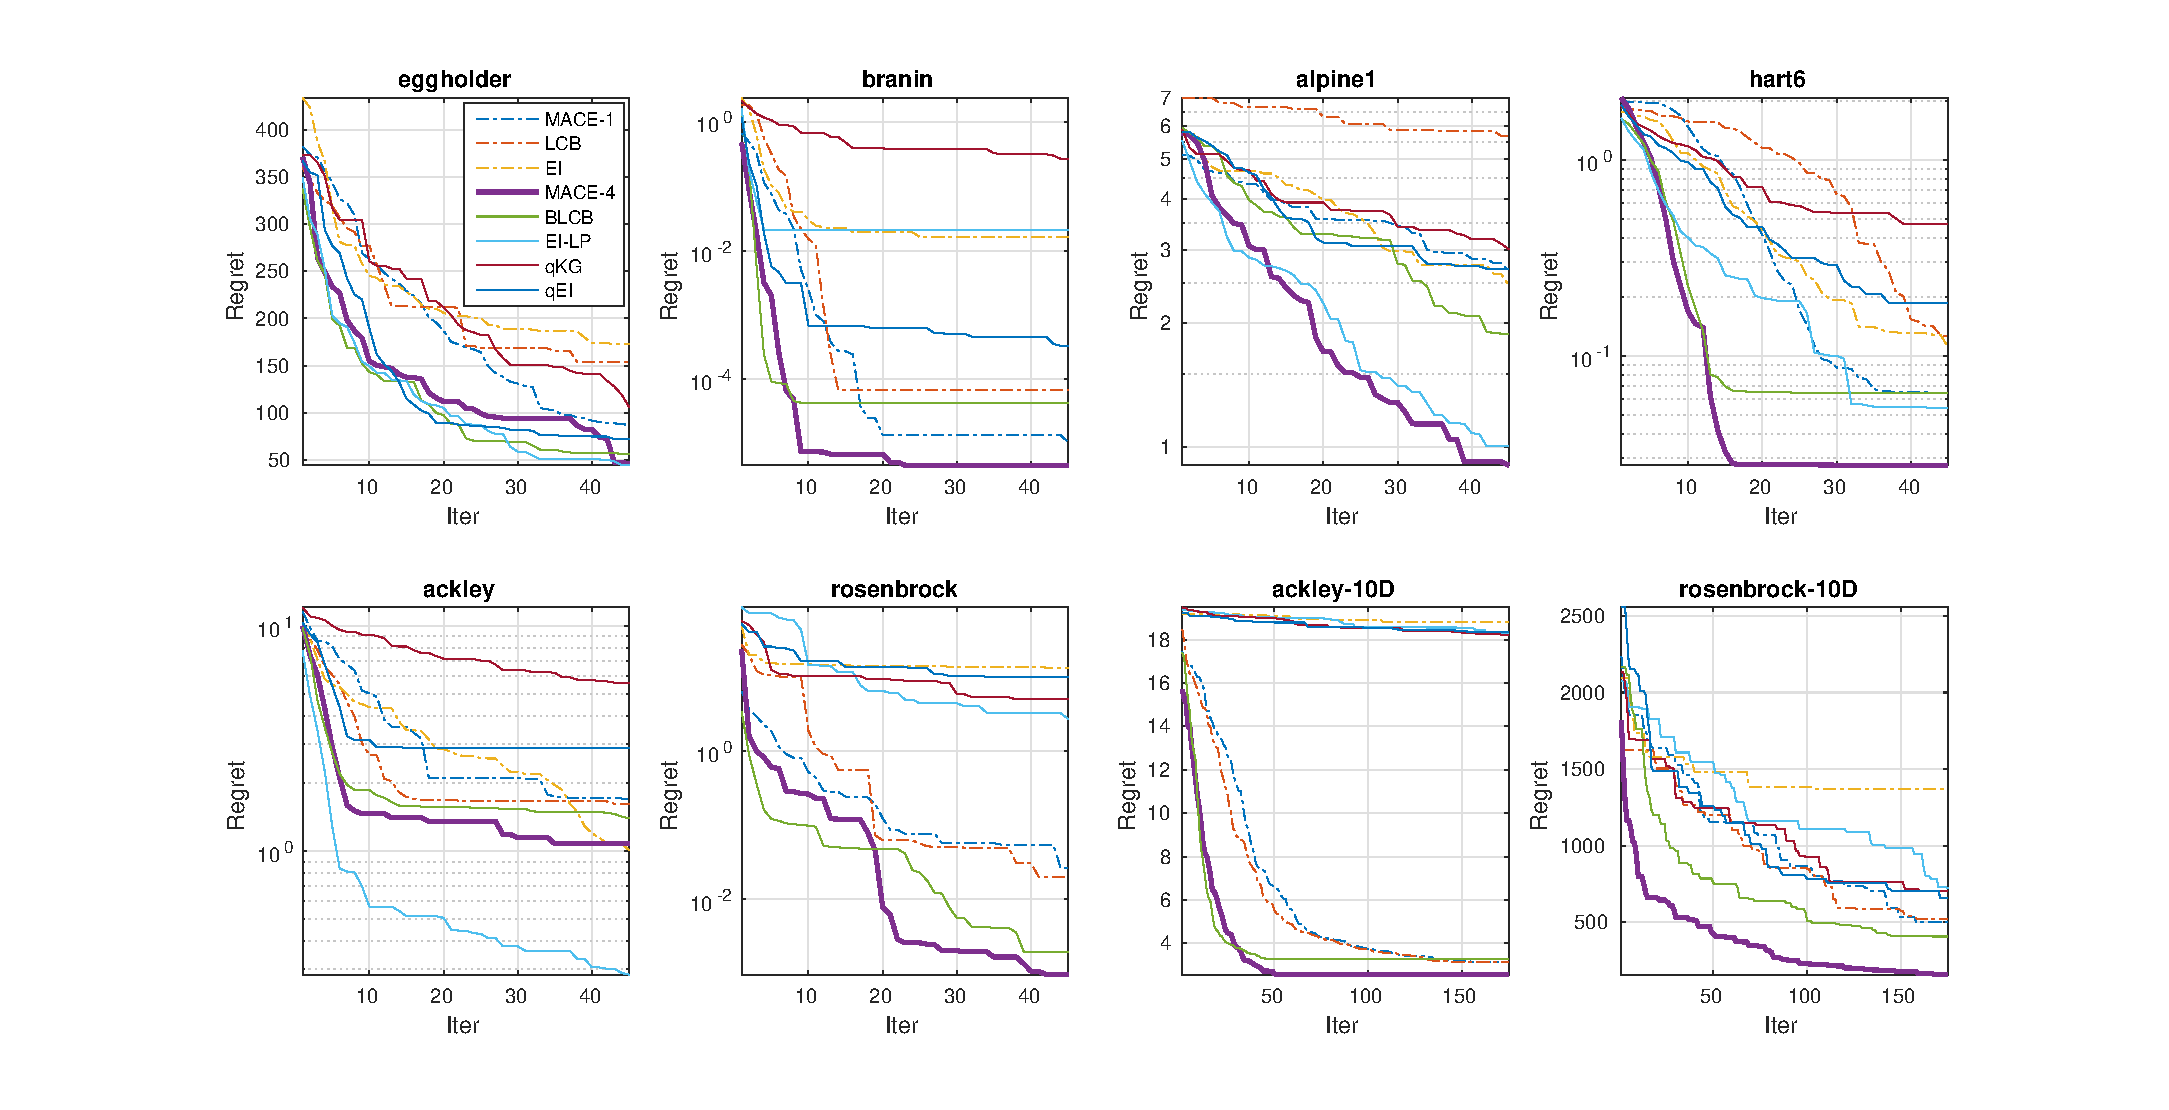
\includegraphics[width=\linewidth]{./img/convplot.eps}}
        \caption{Optimization results of the benchmark functions\textcolor{red}{data still incomplete}}
        \label{fig:CovPlotBenchmark}
    \end{center}
    \vskip -0.2in
\end{figure*}

As can be seen in Figure~\ref{fig:CovPlotBenchmark}, the MACE strategy is
competitive in both sequential and batch setting. The qKG method performed not
good for these benchmark functions, in some functions, it was even outperformed
by the sequential EI and LCB. 

Other algorithms gave acceptable solutions, while the MACE algorithm are
usually the best or second best algorithms for these benchmark functions.

% \begin{table*}[htbp]
%     \centering
%     \caption{Optimization results of the benchmark functions\textcolor{red}{Alert: data still incomplete}}
%     \label{tab:result_analytical}
%     \begin{tabular}{lllllllllll}
%         \toprule
%         Function           & MACE-1             & LCB-1             & EI-1            & MACE-4             & BLCB-4  & EI-LP-4 & qKG-4 & qEI-4  \\ \midrule
%          Branin            & 0.3979$\pm$1.31e-5 & 0.3980$\pm$1.1e-4 & 0.414$\pm$0.016 & 0.3979$\pm$6.64e-6 &         &         &       &        \\
%          Alpine1           & 2.66$\pm$1.06      & 5.67$\pm$1.77     & 2.46$\pm$1.56   &                    &         &         &       &        \\
%          Hartmann6         & -3.26$\pm$0.06     & -3.20$\pm$0.12    & -3.21$\pm$0.15  &                    &         &         &       &        \\
%          Ackley2           & 1.72$\pm$1.12      & 1.62$\pm$0.926    & 1.01$\pm$0.98   &                    &         &         &       &        \\
%          Rosenbrock2       & 0.03$\pm$0.05      & 0.03$\pm$0.02     & 13.55$\pm$9.527 &                    &         &         &       &        \\
%          Ackley10          &                    &                   &                 &                    &         &         &       &        \\
%          Rosenbrock10      &                    &                   &                 &                    &         &         &       &        \\
%         \bottomrule
%     \end{tabular}
% \end{table*}

\subsection{Operational Amplifier}

\textcolor{red}{TODO: qKG and qEI}

\begin{figure}[htbp]
\vskip 0.2in
\begin{center}
\centerline{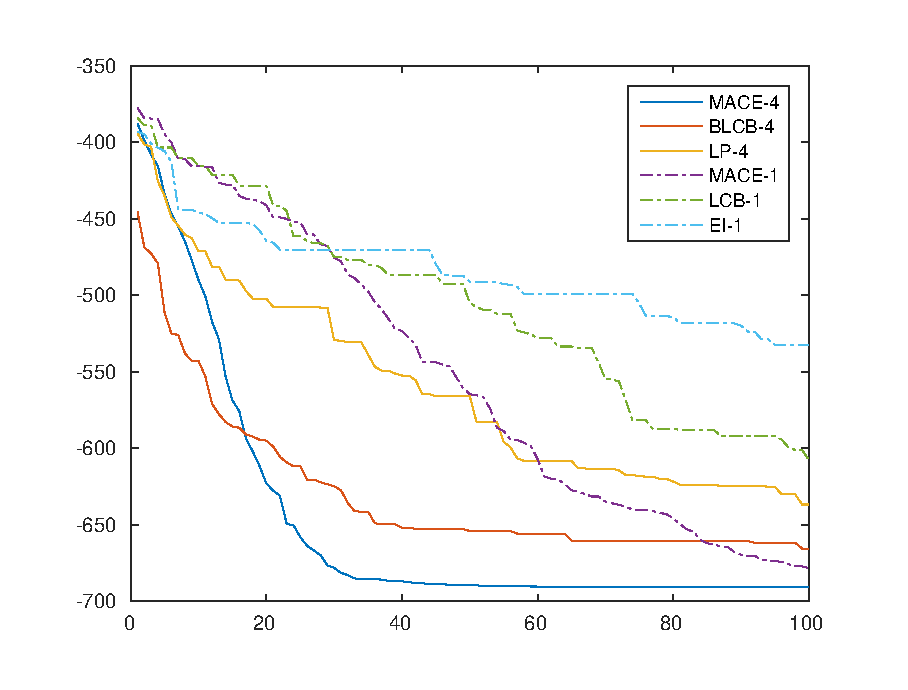
\includegraphics[width=\columnwidth]{./img/mean_DAC2014.eps}}
\caption{Optimization results of the operational amplifier}
\label{resDAC2014}
\end{center}
\vskip -0.2in
\end{figure}


\subsection{ClassE Power Amplifier}

\textcolor{red}{TODO: qKG and qEI}

\begin{figure}[htbp]
\vskip 0.2in
\begin{center}
\centerline{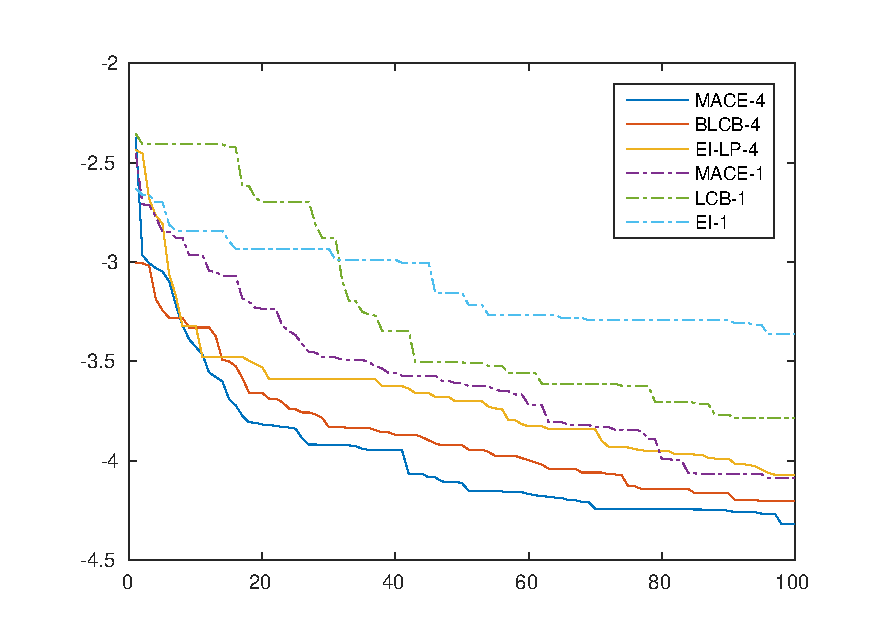
\includegraphics[width=\columnwidth]{./img/ClassE_mean.eps}}
\caption{Optimization results of the class-E power amplifier}
\label{resDAC2014}
\end{center}
\vskip -0.2in
\end{figure}


\FloatBarrier
